\documentclass{scrartcl}
\usepackage{geometry}
\geometry{
	paper=a4paper, 
	top=2.5cm,
	bottom=2.5cm,
	left=2.5cm, 
	right=2.4cm, 
	headheight=0.75cm, 
	footskip=1.5cm, 
	headsep=0.75cm,
}
\usepackage{blindtext}
\usepackage[T1]{fontenc}
\usepackage[utf8]{inputenc}
\usepackage{amsmath, amsfonts, amsthm, amssymb}
\usepackage{braket, nicefrac}
\usepackage{siunitx}
\usepackage{enumitem, multicol}
\usepackage{graphicx, float}  
\usepackage{keystroke}
\usepackage{pgfplots}\usepgfplotslibrary{units}\pgfplotsset{compat=1.16}
\usepackage{setspace}
\usepackage[hidelinks]{hyperref}
\graphicspath{{graphics/}{Graphics/}{./}}
\usepackage{wrapfig}
\usepackage{algorithmicx}
\usepackage{algpseudocode}
\usepackage{algorithm}
\algdef{SE}[DOWHILE]{Do}{doWhile}{\algorithmicdo}[1]{\algorithmicwhile\ #1}



\begin{document}

\begin{titlepage}
	\centering
	
\includegraphics[width=0.6\textwidth]{Graphics/Concordia.png}\par
	\vspace{2cm}
	
	{\scshape\LARGE Software Engineering Processes \par}      
	\vspace{1cm}
	{\scshape\Large Project Report - August 2022\par}
	\vfill
	
	{\huge\bfseries Standard Deviation ($\sigma$)\par}
	\vspace{0.75cm}
	
	{\Large\itshape Kary Sureshbhai Sutariya}\par
	\vspace{0.75cm}
	{\Large\itshape Student Id: 40193909}\par
	\vspace{1.5cm}

	\vfill
	{\Large\itshape supervised by}\par
	\vspace{0.5cm}

	{\Large\itshape Dr. Pankaj Kamthan}\par
	\vspace{1.5cm}
	 


	\vfill
\end{titlepage}

\newpage

\singlespacing

% \section{Introduction}
% \begin{Large}
% In this project, Standard deviation function is going to be center of discussion. What are the domains and co-domains of the function will be covered in detail. Furthermore, there will be a small section for the characteristic of the function. Later on, user model will be made so all types of users can use this function. 
% \end{Large}

\section{Problem 1}
\subsection{Description}
\begin{Large}
Standard deviation is the square root of variance and variance provides variability from the mean. Standard deviation is denoted by a Greek symbol $\sigma$. The equation for Standard deviation is given below.[\ref{key1}] 

\begin{center}
\vspace{0.2cm}
\begin{Large}
$\sigma = \sqrt{\frac{1}{N} \sum_{i=1}^N (x_i - \overline{x})^2}$
\end{Large}
\end{center}

where:

${x_i}$: Each value in the data set

$\overline{x}$: Mean of all values in the data set

N: Number of values in the data set

\begin{wrapfigure}{r}{0.5\textwidth}
    \centering
    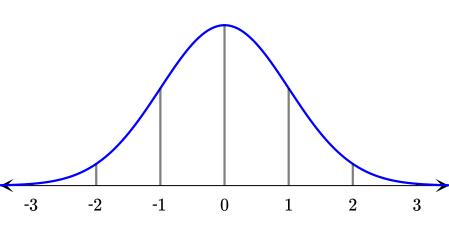
\includegraphics[width=0.5\textwidth]{Graphics/sd.png}
    \caption{Graph of Standard deviation [\ref{key2}]}
    \label{fig:Graph of Standard deviation}
\end{wrapfigure}

\vspace{0.2cm}
Figure \ref{fig:Graph of Standard deviation} shows normal curve standard deviation. In this case, values are distributed equally over the range. This type of distribution is ideal for many real-time projects. For instance, data scientists always try to make their data set equally distributed and to check it, standard deviation has been utilized over the time again and again. 

\end{Large}

\subsection{Domain and Co-domain}
\begin{Large}
For Standard deviation, all real numbers are in its domain and co-domain. Real number ${\displaystyle (\mathbb {R} )}$ includes rational numbers ${\displaystyle (\mathbb {Q} )}$, which include the integers ${\displaystyle (\mathbb {Z} )}$, which in turn include the natural numbers ${\displaystyle (\mathbb {N} )}$ but not imaginary numbers${\displaystyle ( {i} )}$.[\ref{key3}] In the mathematical term, It can be written like this. 

\begin{center}
$\sigma: {\displaystyle \mathbb {R}} \rightarrow {\displaystyle \mathbb {R}}$
\end{center}

\end{Large}

\subsection{Characteristic}
\begin{Large}
\begin{itemize}
  \item If the Standard deviation is high, numbers are scattered far from each other.
  \item Whereas if numbers are nearby to each other, the Standard deviation will be low. 
  \item It is sensitive to extreme values. A small change in any extreme value can lead to drastic alteration.[\ref{key4}]
\end{itemize}
\end{Large}

\newpage

\subsection{Use model}

In this section, context of use model has been explained. The following Use model depicts where the standard deviation function can be used by users. Standard deviation is being used in various fields namely AI, Finance, Resource management, Environmental studies etc. 

\begin{figure}[H]
    \centering
    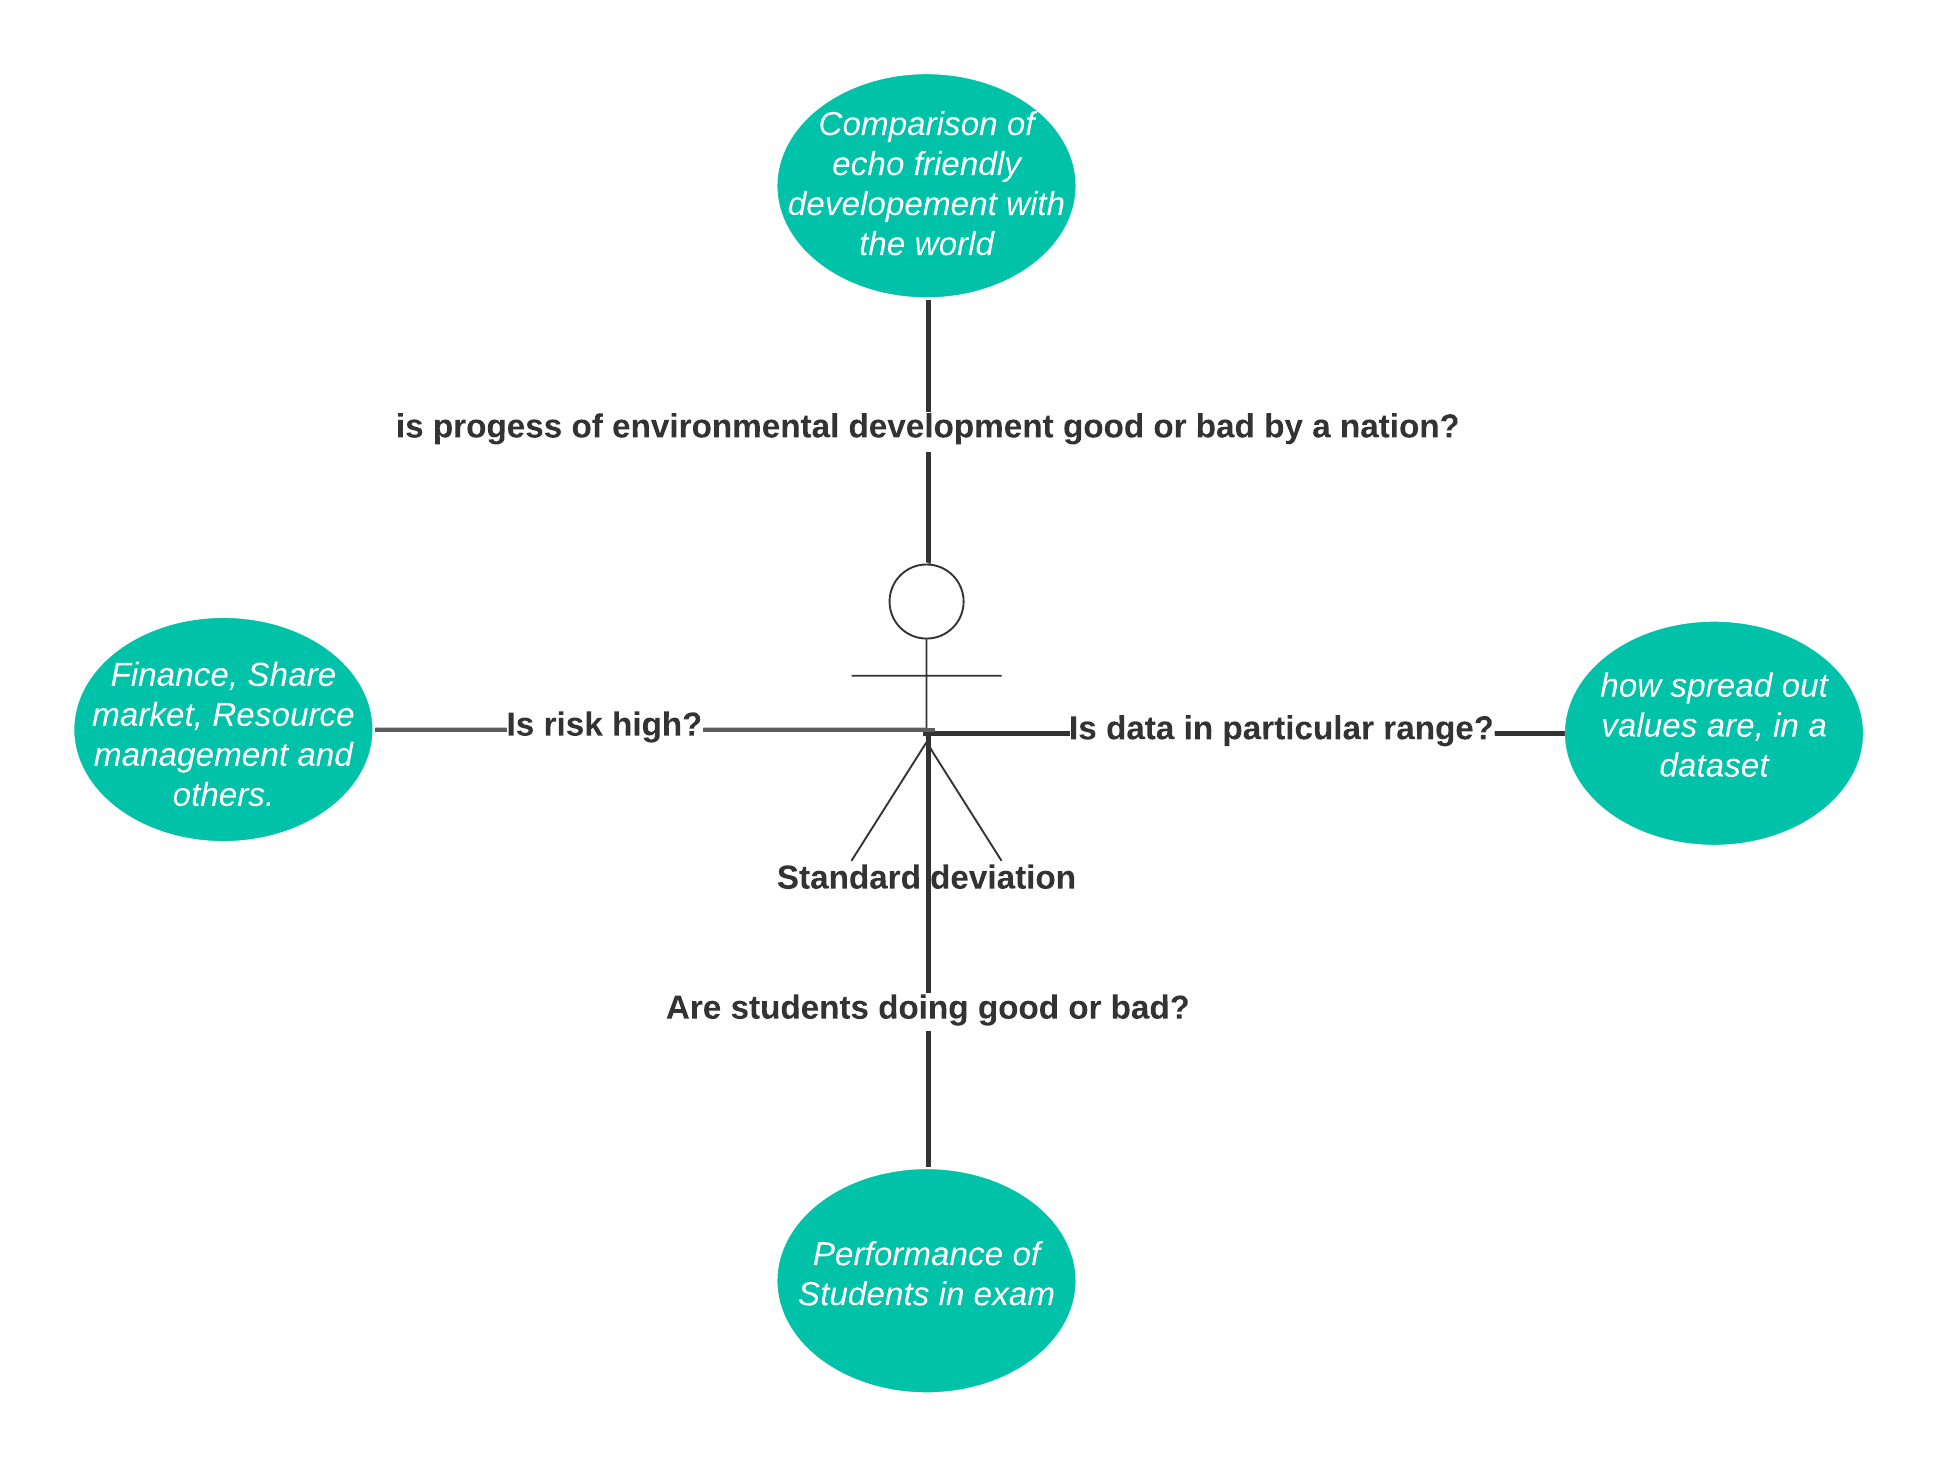
\includegraphics[width=1\textwidth]{Graphics/usecase.png}
    \caption{Use model}
    \label{fig:usemodel}
\end{figure}

\newpage

\section{Problem 2}

\vspace{0.5cm}
\subsection{First Requirement}

\begin{LARGE}
\begin{itemize}
  \item \textbf{ID:} FR 1 
  \item \textbf{Type:} Functional Requirement 
  \item \textbf{Version:} 1.0
  \item \textbf{Priority:} Highest
  \item \textbf{Description:} Since standard deviation tells how close the numbers are, all the inputs must be numbers and not a character or set of characters.
\end{itemize}
\end{LARGE}

\subsection{Second Requirement}

\begin{LARGE}
\begin{itemize}
  \item \textbf{ID:} FR 2 
  \item \textbf{Type:} Functional Requirement 
  \item \textbf{Version:} 1.0
  \item \textbf{Priority:} Low
  \item \textbf{Description:} To calculate the mean, all real numbers must be considered.
\end{itemize}
\end{LARGE}

\subsection{Third Requirement}

\begin{LARGE}
\begin{itemize}
  \item \textbf{ID:} FR 3 
  \item \textbf{Type:} Functional Requirement 
  \item \textbf{Version:} 1.0
  \item \textbf{Priority:} High
  \item \textbf{Description:} Standard deviation must not have to be negative as it is the square root of variance.
\end{itemize}
\end{LARGE}

\subsection{Fourth Requirement}

\begin{LARGE}
\begin{itemize}
  \item \textbf{ID:} FR 4 
  \item \textbf{Type:} Functional Requirement 
  \item \textbf{Version:} 1.0
  \item \textbf{Priority:} Medium 
  \item \textbf{Description:} If variance exists, Standard deviance exists and vice versa.   
\end{itemize}
\end{LARGE}

\subsection{Fifth Requirement}

\begin{LARGE}
\begin{itemize}
  \item \textbf{ID:} FR 5 
  \item \textbf{Type:} Non-Functional Requirement (System)
  \item \textbf{Version:} 1.0
  \item \textbf{Priority:} Medium 
  \item \textbf{Description:} Higher availability of memory will result in swift execution when total input numbers are high.    
\end{itemize}
\end{LARGE}

\subsection{Sixth Requirement}

\begin{LARGE}
\begin{itemize}
  \item \textbf{ID:} FR 6
  \item \textbf{Type:} Non-Functional Requirement (Portability) 
  \item \textbf{Version:} 1.0
  \item \textbf{Priority:} High 
  \item \textbf{Description:} Java virtual machine (JVM) is a virtual machine that enables a computer to run the program.
\end{itemize}
\end{LARGE}

\newpage

\section{Problem 3}

\subsection{Pseudo Code for Iterative approach}

\begin{algorithm}
\caption{Standard Deviation with iterative}\label{alg:Standard Deviation with iterative}
\begin{algorithmic}
\Function{main}{}
    \State $N \gets n$
    \State $x[N] \gets  = {1, 5, ..., n^{\text{th}}\ number}$
    \State $\overline{x} = \Call{cal\_mean}{x[N],N}$
    \State $var = \Call{variance}{x[N],N,\overline{x}}$
    \State $\sigma = \Call{sqrt}{var}$
\EndFunction
\Function{cal\_mean}{$x[N],N$}
    \State $avg \gets 0$
    \For{$i \gets 1$ to $N$} 
        \State $avg \gets avg + x[i]$
    \EndFor
    \State \textbf{return} {$avg / N$} 
\EndFunction
\Function{square}{$number$} 
    \State \textbf{return} {$number * number$} 
\EndFunction
\Function{sqrt}{$number$}
    \If{$number != 0$} 
        \State $T \gets 0$
        \State $sqrtRoot \gets T/2$
        \Do
            \State $T \gets sqrtRoot$
            \State $sqrtRoot \gets (T + (number/T)/2$
        \doWhile{$(T-sqrtRoot) != 0$}
        \State \textbf{return} {sqrtRoot}
    \Else
       \State \textbf{return} {0} 
    \EndIf 
\EndFunction
\Function{variance}{$x[N],N,avg$}
    \State $temp \gets 0$
    \For{$i \gets 1$ to $N$} 
        \State $temp \gets temp + \Call{square}{x[i] - avg}$
    \EndFor 
    \State \textbf{return} {temp / N}
\EndFunction
\end{algorithmic}
\end{algorithm}

\begin{spacing}{1.5}
\begin{Large}
There are a total of 4 subordinate functions and one main function. In the above algorithm, $\Call{cal\_mean}{x[N],N}$ and $\Call{variance}{x[N],N,\overline{x}}$ functions have been defined using an iterative approach.  
\end{Large}
\end{spacing}

\subsection{Pseudo Code for Recursive approach}

\begin{algorithm}[H]
\caption{Standard Deviation with recursion}\label{alg:Standard Deviation with recursion}
\begin{algorithmic}
\Function{main}{}
    \State $N \gets n$
    \State $k \gets 0$
    \State $x[N] \gets  = {1, 5, ..., n^{\text{th}}\ number}$
    \State $\overline{x} = \Call{cal\_mean}{x[N],k,N}$
    \State $var = \Call{variance}{x[N],N,k,\overline{x}}$
    \State $\sigma = \Call{sqrt}{var}$
\EndFunction
\Function{cal\_mean}{$x[N],k, N$}
    \If{$k == N$} 
        \State $avg \gets avg / N$
        \State \textbf{return} {avg}
    \Else
       \State $avg \gets avg + x[k]$
       \State $k++$
       \State \textbf{return} \Call{cal\_mean}{$x[N],k, N$}
    \EndIf 
\EndFunction
\Function{square}{$number$} 
    \State \textbf{return} {$number * number$} 
\EndFunction
\Function{sqrt}{$number$}
    \If{$number != 0$} 
        \State $T \gets 0$
        \State $sqrtRoot \gets T/2$
        \Do
            \State $T \gets sqrtRoot$
            \State $sqrtRoot \gets (T + (number/T)/2$
        \doWhile{$(T-sqrtRoot) != 0$}
        \State \textbf{return} {sqrtRoot}
    \Else
       \State \textbf{return} {0} 
    \EndIf 
\EndFunction
\Function{variance}{$x[N],N,k,avg,var=0$}
    \If{$k == N$} 
        \State $var \gets var / N$
        \State \textbf{return} {var}
    \Else
       \State $var \gets \Call{square}{x[k] - avg}$
       \State $k++$
       \State \textbf{return} \Call{variance}{$x[N],N,k,avg,var$}
    \EndIf 
\EndFunction
\end{algorithmic}
\end{algorithm}
\begin{spacing}{1.5}
\begin{Large}
For Recursive algorithm, $\Call{cal\_mean}{x[N],N}$ and $\Call{variance}{x[N],N,\overline{x}}$ functions have been made recursive approach
whereas $\Call{square}{number}$ and $\Call{sqrt}{number}$, both the 
functions are similar in both the algorithms.
\end{Large}
\end{spacing}

\subsection{Mind map}

\begin{spacing}{1.5}
\begin{Large}
The below mind map helps to understand how all the subordinate functions will be executed by algorithms. Mind map for both is same. The reason for that is same structure has been used. The inner approach and the number of arguments are different for subordinate functions. Execution of algorithms will start from the main function. Next, $\Call{cal\_mean}$ will be called to calculate mean and this mean will be passed to $\Call{variance}$. Moreover, $\Call{variance}$ will use $\Call{square}$ function to calculate the square of numbers. In the last, $\Call{sqrt}$ will be called to get square root of the variance and it will give the standard deviation. 
\end{Large}
\end{spacing}

\begin{figure}[H]
    \centering
    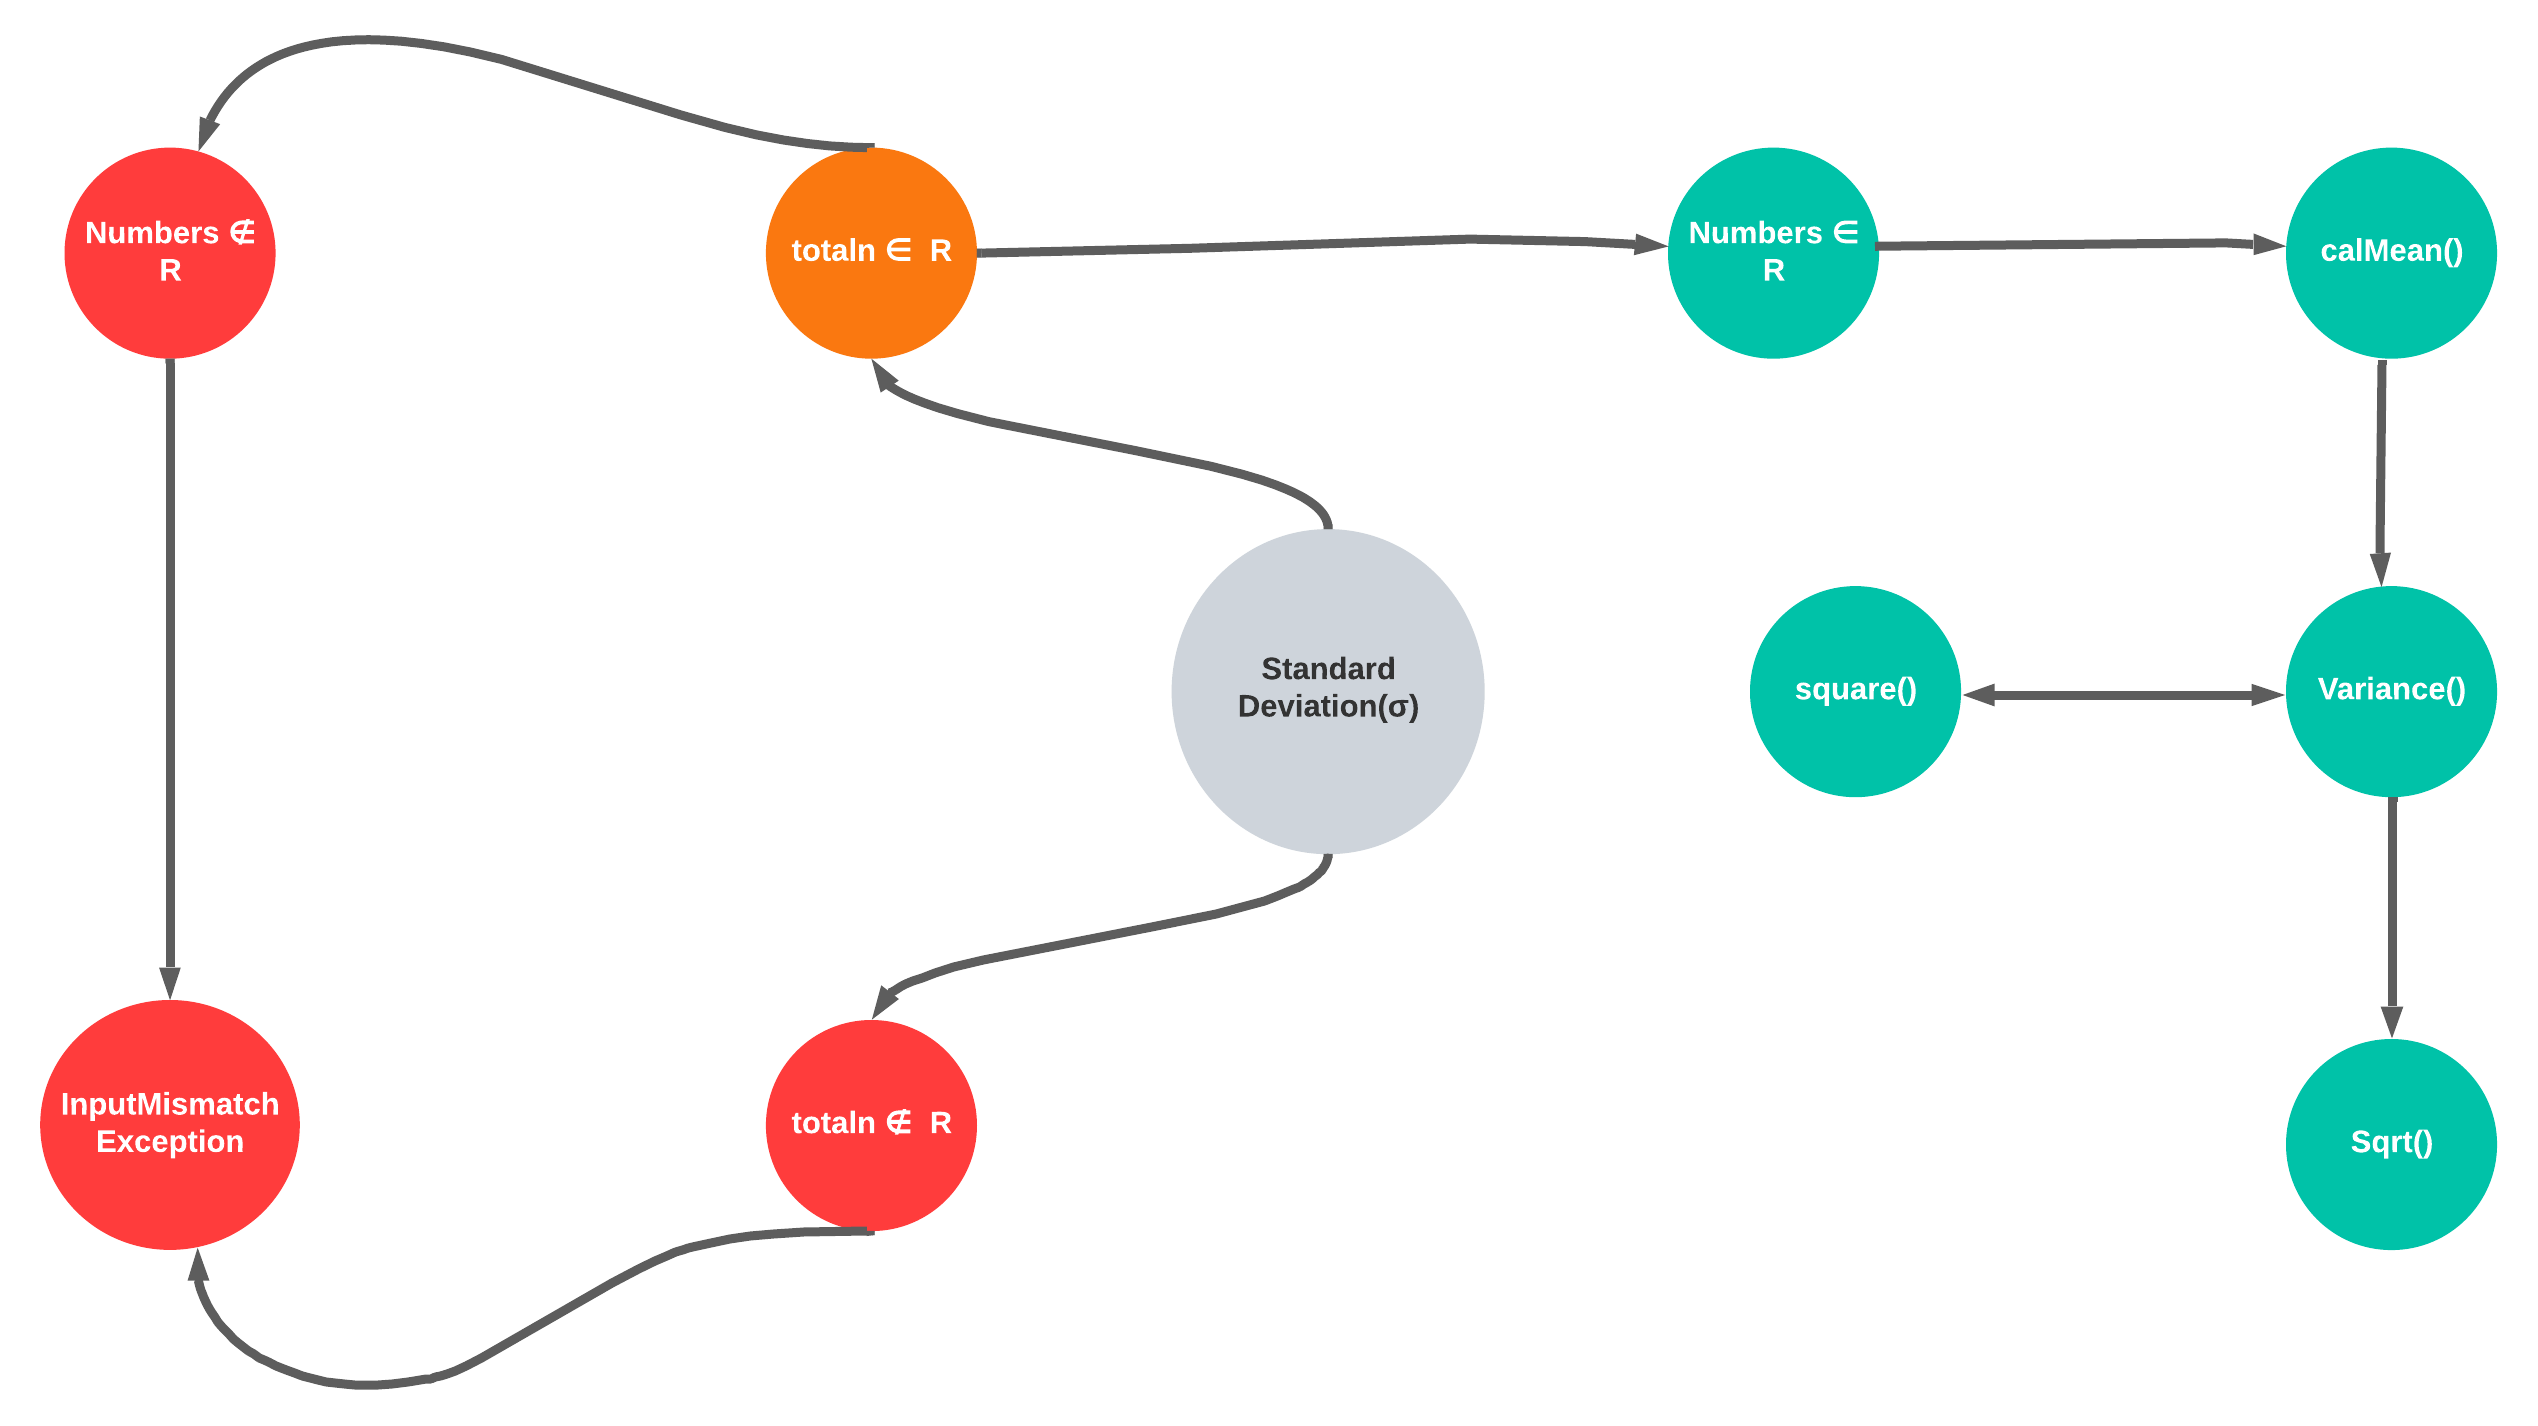
\includegraphics[width=1\textwidth]{Graphics/mindmap.png}
    \caption{mindmap}
    \label{fig:mindmap}
\end{figure}



\subsection{Iterative Algorithm}

\begin{spacing}{1.5}
\begin{Large}
\textbf{Reason to opt Iterative approach:} 
Iterative approach is less dependent on memory and more on computation power of the system. To get results with less space availability, this approach has been implemented in this project.
\end{Large}
\end{spacing}

\newpage

\begin{Large}
\vspace{0.8cm}
\textbf{Pros:}
\begin{itemize}
  \item It doesn't generate overhead.
  \item Never will face the problem of Stack overflow.
  \item Easy to explain to even children want to learn to code.
\end{itemize}
\end{Large}

\begin{Large}
\vspace{0.5cm}
\textbf{Cons:}
\begin{itemize}
  \item For large input, calculation time will be higher.
  \item Doesn't utilization memory up to the mark which will lead to slow execution.[\ref{key5}]
\end{itemize}
\end{Large}

\subsection{Recursive Algorithm}

\begin{spacing}{1.5}
\begin{Large}
\textbf{Reason to opt Recursive approach:} 
Recursion is totally dependent on memory and will can give faster execution. Also, to analyze how use of more memory can play a vital role in the execution of code.
\end{Large}
\end{spacing}

\begin{Large}
\vspace{0.5cm}
\textbf{Pros:}
\begin{itemize}
  \item Fully utilize memory up to the mark for rapid execution.
  \item It is suitable for the small size of the input.
\end{itemize}
\end{Large}

\begin{Large}
\vspace{0.5cm}
\textbf{Cons:}
\begin{itemize}
  \item For large input, it is slow and maybe, it can produce stack over error.
  \item Complex to understand. 
  \item generates overhead during execution. 
  Doesn't utilization memory up to the mark which will lead to slow execution. [\ref{key6}]
\end{itemize}
\end{Large}

\newpage

\section{Problem 4}

\begin{spacing}{1.5}
\begin{Large}
The standard deviation function has been implemented in pure Java applications. Moreover, it is compatible with Eclipse and IntelliJ. However, High-end user can run it from the command line. More details are available in ’Readme.md’ file.
\end{Large}
\end{spacing}

\subsection{Error Handling}

\begin{spacing}{1.5}
\begin{Large}
Human is to err. As said that, there is a chance for wrong input from a user. To handle that, the Input Mismatch Exception has been used in the code for total numbers and numbers.  
\end{Large}
\end{spacing}

\subsection{Error Messaging}

\begin{spacing}{1.5}
\begin{Large}
Error messages are paramount. Many times developers use Systemoutprintln in the production phase. This is a wrong practice performed by the coder but here, logger function of java.util library has been used to pass error messages. As well as the program will log appropriate messages in such conditions.
\end{Large}
\end{spacing}

\subsection{Debugger}

\begin{spacing}{1.5}
\begin{Large}
A debugger is a special tool often used programmers to find out bugs.[\ref{key7}] All high level language code can be easily debugged. Find out bugs can be a tedious task but it also depended on the skills of the programmer. In this project, the debugger has been used as shown in Figure \ref{fig:debug}.  
\end{Large}
\end{spacing}

\begin{Large}
\vspace{0.5cm}
\textbf{Pros:}
\begin{itemize}
  \item For any programmer, it is not possible to able to think about all corner cases and debugger can help in these situations. 
  \item Able to modify values at run time.
  \item User can put any number of breakpoints to evaluate certain sections of program. 
  \item To see the flow of control. 
\end{itemize}
\end{Large}

\begin{figure}[H]
    \centering
    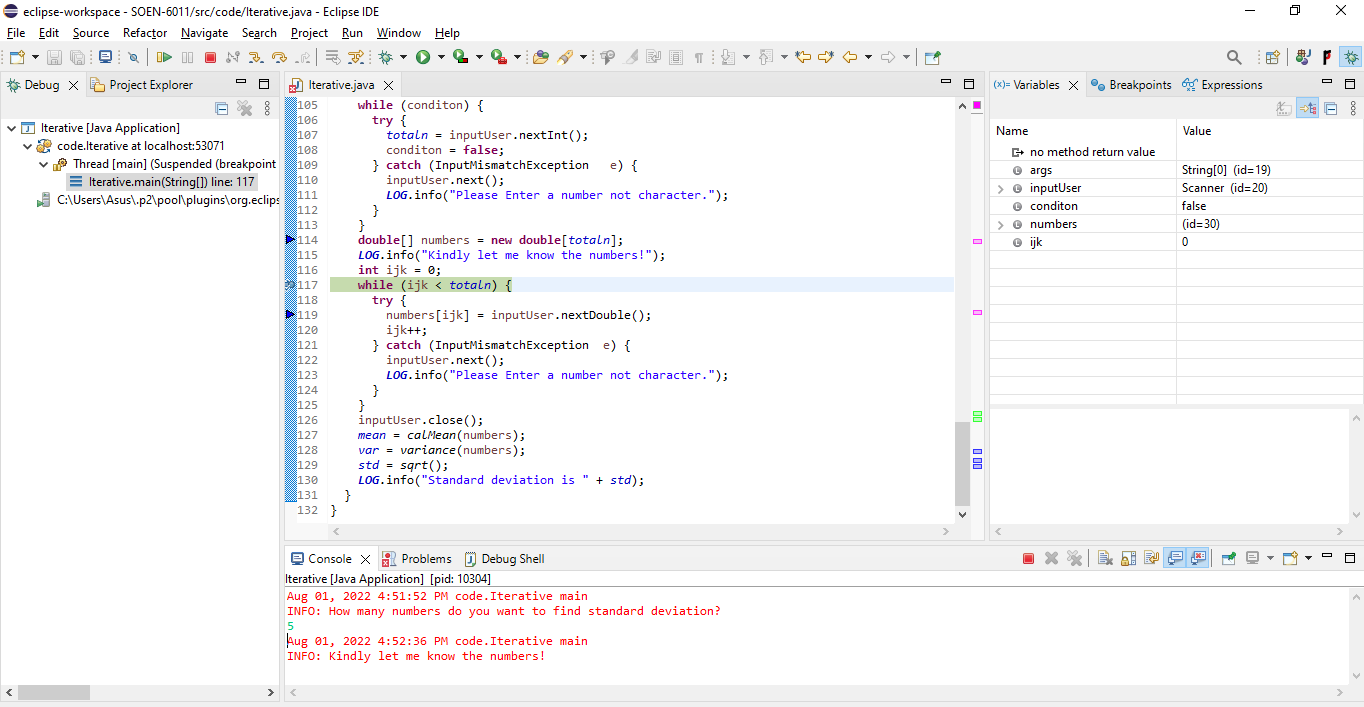
\includegraphics[width=1\textwidth]{Graphics/debug.png}
    \caption{Screenshot of debugger}
    \label{fig:debug}
\end{figure}

\begin{Large}
\vspace{0.5cm}
\textbf{Cons:}
\begin{itemize}
  \item With different IDES, debugging process is different.   
  \item Doesn't provide a 'Rollback' feature.
\end{itemize}
\end{Large}

\vspace{0.2cm}
\subsection{Pragmatic Quality Checking Tool}

\begin{spacing}{1.5}
\begin{Large}
Quality checking helps to increase the quality of code so in future if other programmer tries to upgrade or understand code, he/she doesn't face any problems. There are many Pragmatic Quality Checking Tools. The one which one used in this project is the below. This one is available on Eclipse Market place.

\textbf{Name of Tool:} eclipse-cs[\ref{key8}]

\textbf{Standards:} Sun Code Conventions and Google Java Style.

\textbf{Version:} 10.3.2

\textbf{Published By:} Lars ödderitzsch

\end{Large}
\end{spacing}

\begin{figure}[H]
    \centering
    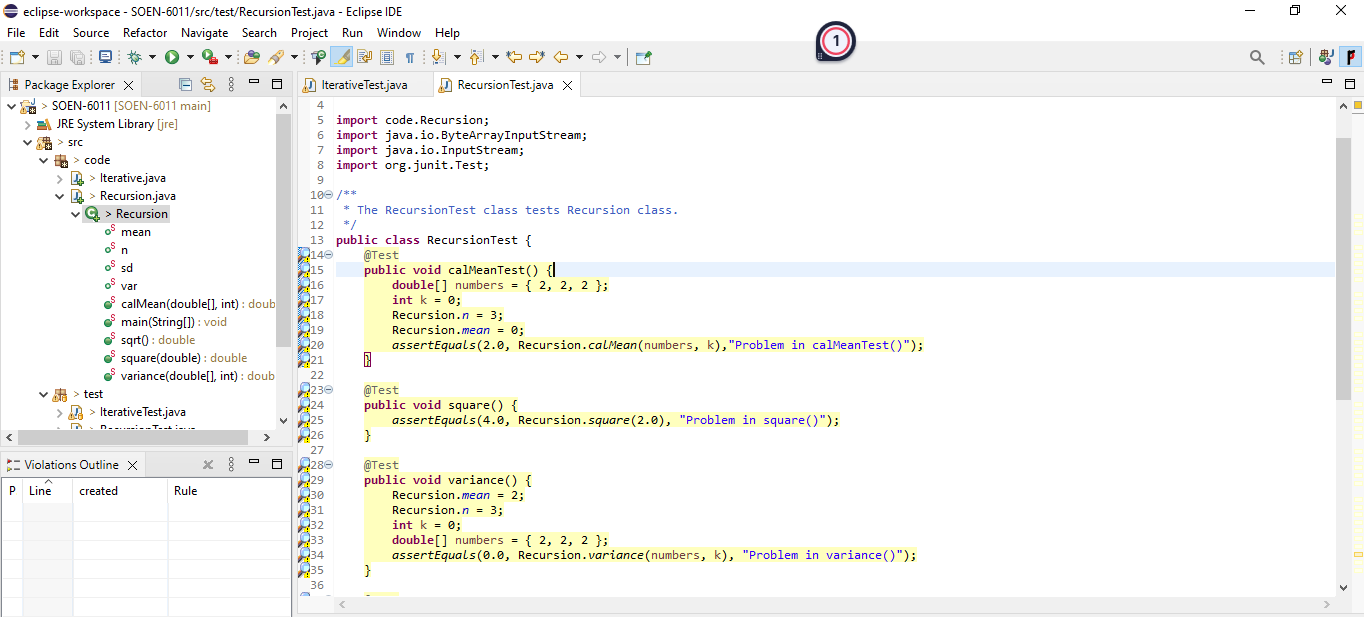
\includegraphics[width=1\textwidth]{Graphics/check style.png}
    \caption{Screen shot of check style}
    \label{fig:check style}
\end{figure}

\begin{Large}
\vspace{0.5cm}
\textbf{Pros:}
\begin{itemize}
  \item Can easily integrate with different IDES.  
  \item User can add custom rules.  
  \item Bring unification to a team project. 
\end{itemize}
\end{Large}

\begin{Large}
\vspace{0.5cm}
\textbf{Cons:}
\begin{itemize}
  \item Frequent recompile is required.
  \item Because of cache, sometimes even if the problem has been solved but it shows there is one. 
  \item Simple rules can lead to large changes. 
  \item Doesn't improve the quality of code like PMD tool. 
\end{itemize}
\end{Large}

\newpage

\section{Problem 5}

\begin{spacing}{1.5}
\begin{Large}
All unit test cases for Standard Deviation ($\sigma$) ensure that functions work as expected when given various kinds of inputs. For this tedious task, Junit framework has utilized. It helps to figure out the actual behaviour of code in a kind of simulated situation.   
\end{Large}
\end{spacing}

\subsection{Standards for unit tests}

\begin{spacing}{1.5}
\begin{Large}
In the project, to check the standard of unit tests Check-Style plug-in has been used. Initially, these unit tests have problems like multiple assert statements in one unit test which had been separated into different unit cases like sqrtTest1() and sqrtTest2(). Adding to that, all the test cases are traceable to requirements. 
\end{Large}
\end{spacing}

\subsection{Unit case traceability with requirements}
\begin{spacing}{1.5}
\begin{Large}
Each and every test case is intertwined with one of the requirements. There is one to one relationship between test cases and requirements. More details can be captured from the following tables.  
\end{Large}
\end{spacing}

\begin{table}[H]
\begin{Large}
\begin{center}
\begin{tabular}{ | m{10em} | m{10em} | } 
  \hline
  \multicolumn{2}{|c|}{\textbf {Unit Test 1}} \\ 
  \hline
  \textbf{Test Case ID}  &  TR 1\\ 
  \hline
  \textbf{Requirement ID} &  FR 1\\
  \hline
  \textbf{Name of test case} & mainTest()\\
  \hline
  \textbf{Input(s) } &  c 2 2 g 2 \\
  \hline
  \textbf{Expected Output } & 0\\
  \hline
  \textbf{Actual Output } & 0\\
  \hline
  \textbf{Test Result } & Success \\
 \hline
\end{tabular}
\caption{Unit test for requirement 1}
\label{table:unit test 1}
\end{center}
\end{Large}
\end{table}

\begin{table}[H]
\begin{Large}
\begin{center}
\begin{tabular}{ | m{10em} | m{10em} | } 
  \hline
  \multicolumn{2}{|c|}{\textbf {Unit Test 2}} \\ 
  \hline
  \textbf{Test Case ID}  &  TR 2\\ 
  \hline
  \textbf{Requirement ID} &  FR 2\\
  \hline
  \textbf{Name of test case} & calMeanTest()\\
  \hline
  \textbf{Input(s) } &  2 2 2 \\
  \hline
  \textbf{Expected Output } & 0\\
  \hline
  \textbf{Actual Output } & 0\\
  \hline
  \textbf{Test Result } & Success \\
 \hline
\end{tabular}
\caption{Unit test for requirement 2}
\label{table:unit test 2}
\end{center}
\end{Large}
\end{table}

\begin{table}[H]
\begin{Large}
\begin{center}
\begin{tabular}{ | m{10em} | m{10em} | } 
  \hline
  \multicolumn{2}{|c|}{\textbf {Unit Test 3.1}} \\ 
  \hline
  \textbf{Test Case ID}  &  TR 3.1\\ 
  \hline
  \textbf{Requirement ID} &  FR 3\\
  \hline
  \textbf{Name of test case} & sqrtTest1()\\
  \hline
  \textbf{Input(s) } &  0.0 \\
  \hline
  \textbf{Expected Output } & 0\\
  \hline
  \textbf{Actual Output } & 0\\
  \hline
  \textbf{Test Result } & Success \\
 \hline
\end{tabular}
\caption{Unit test for requirement 3}
\label{table:unit test 3.1}
\end{center}
\end{Large}
\end{table}

\begin{table}[H]
\begin{Large}
\begin{center}
\begin{tabular}{ | m{10em} | m{10em} | } 
  \hline
  \multicolumn{2}{|c|}{\textbf {Unit Test 3.2}} \\ 
  \hline
  \textbf{Test Case ID}  &  TR 3.2\\ 
  \hline
  \textbf{Requirement ID} &  FR 3\\
  \hline
  \textbf{Name of test case} & sqrtTest2()\\
  \hline
  \textbf{Input(s) } &  4.0 \\
  \hline
  \textbf{Expected Output } & 2.0\\
  \hline
  \textbf{Actual Output } & 2.0\\
  \hline
  \textbf{Test Result } & Success \\
 \hline
\end{tabular}
\caption{Unit test for requirement 3}
\label{table:unit test 3.2}
\end{center}
\end{Large}
\end{table}

\begin{table}[H]
\begin{Large}
\begin{center}
\begin{tabular}{ | m{10em} | m{10em} | } 
  \hline
  \multicolumn{2}{|c|}{\textbf {Unit Test 4}} \\ 
  \hline
  \textbf{Test Case ID}  &  TR 4\\ 
  \hline
  \textbf{Requirement ID} &  FR 4\\
  \hline
  \textbf{Name of test case} & variance()\\
  \hline
  \textbf{Input(s) } &  2 2 2\\
  \hline
  \textbf{Expected Output } & 0.0\\
  \hline
  \textbf{Actual Output } & 0.0\\
  \hline
  \textbf{Test Result } & Success \\
 \hline
\end{tabular}
\caption{Unit test for requirement 4}
\label{table:unit test 4}
\end{center}
\end{Large}
\end{table}

\begin{spacing}{1.5}
\begin{Large}
Moving ahead, the requirement 5 and so forth are non-functional requirements so there is no way to write test cases for these non-functional requirements.
\end{Large}
\end{spacing}

\newpage

\section{Bibliography}

\begin{spacing}{1}
\begin{Large}
\begin{enumerate}
    \item \label{key1}\href{https://en.wikipedia.org/wiki/Standard_deviation}{https://en.wikipedia.org/wiki/Standard\_deviation}
    \item \label{key2}\href{https://mathleaks.com/mediawiki/images/5/5a/Mljsx_Concept_standard_distribution_1_old.svg}{https://mathleaks.com/mediawiki/images/5/5a/Mljsx Concept standard distribution 1 old.svg}
    \item \label{key3} \href{https://en.wikipedia.org/wiki/Domain\_of\_a\_function}{https://en.wikipedia.org/wiki/Domain\_of\_a\_function}
    \item \label{key4} \href{https://www150.statcan.gc.ca/n1/edu/power-pouvoir/ch12/5214891-eng.htm}{https://www150.statcan.gc.ca/n1/edu/power-pouvoir/ch12/5214891-eng.htm} 
    \item \label{key5} \href{https://www.dcsl.com/pros-cons-iterative-software-development/}{https://www.dcsl.com/pros-cons-iterative-software-development/}
    \item \label{key6} \href{https://medium.com/@williambdale/recursion-the-pros-and-cons-76d32d75973a}{https://medium.com/@williambdale/recursion-the-pros-and-cons} 
    \item \label{key7} \href{https://docs.oracle.com/javase/7/docs/technotes/tools/windows/jdb.html#:~:text=The\%20Java\%20Debugger\%2C\%20jdb\%2C\%20is,or\%20remote\%20Java\%20Virtual\%20Machine.}{https://docs.oracle.com/javase/7/docs/technotes/tools/windows/jdb.html}
    \item \label{key8} \href{https://checkstyle.org/eclipse-cs/#!/}{https://checkstyle.org/eclipse-cs/\#!/}
\end{enumerate}
\end{Large}
\end{spacing}

\end{document}